% Defino el tipo de documento.
\documentclass[a4paper,11pt]{article}
\usepackage[spanish]{babel}
\usepackage[utf8]{inputenc}
% Este es para poder poner graficos y diagramas.
\usepackage{graphicx}
% Este paquete me permite poner grados celsius.
\usepackage{textcomp}

\title{
        Programación de Objetos Distribuidos \\
        Entrega \#1: \\
        Diagrama y Casos de Uso
    }

\author{
        Grupo 3. \\
        46099 - Abramowicz, Pablo Federico \\
        46281 - Cabral, Martín Esteban \\
        47031 - Gomez, Vidal Darío Maximiliano \\
        46383 - Goñi, Juan Ignacio \\
        46233 - Palombo, Martín \\
        46069 - Sessa, Carlos Manuel
        }
\date{}

% Empieza el documento.
\begin{document}


\maketitle
\pagebreak

%Redefine the first level
\renewcommand{\theenumi}{\arabic{enumi}.}
\renewcommand{\labelenumi}{\theenumi}

%Redefine the second level
\renewcommand{\theenumii}{\arabic{enumii}.}
\renewcommand{\labelenumii}{\theenumii}

%Redefine the thrid level
\renewcommand{\theenumiii}{\arabic{enumiii}.}
\renewcommand{\labelenumiii}{\theenumiii}


\section{Diagrama de Casos de Uso}

\begin{center}
 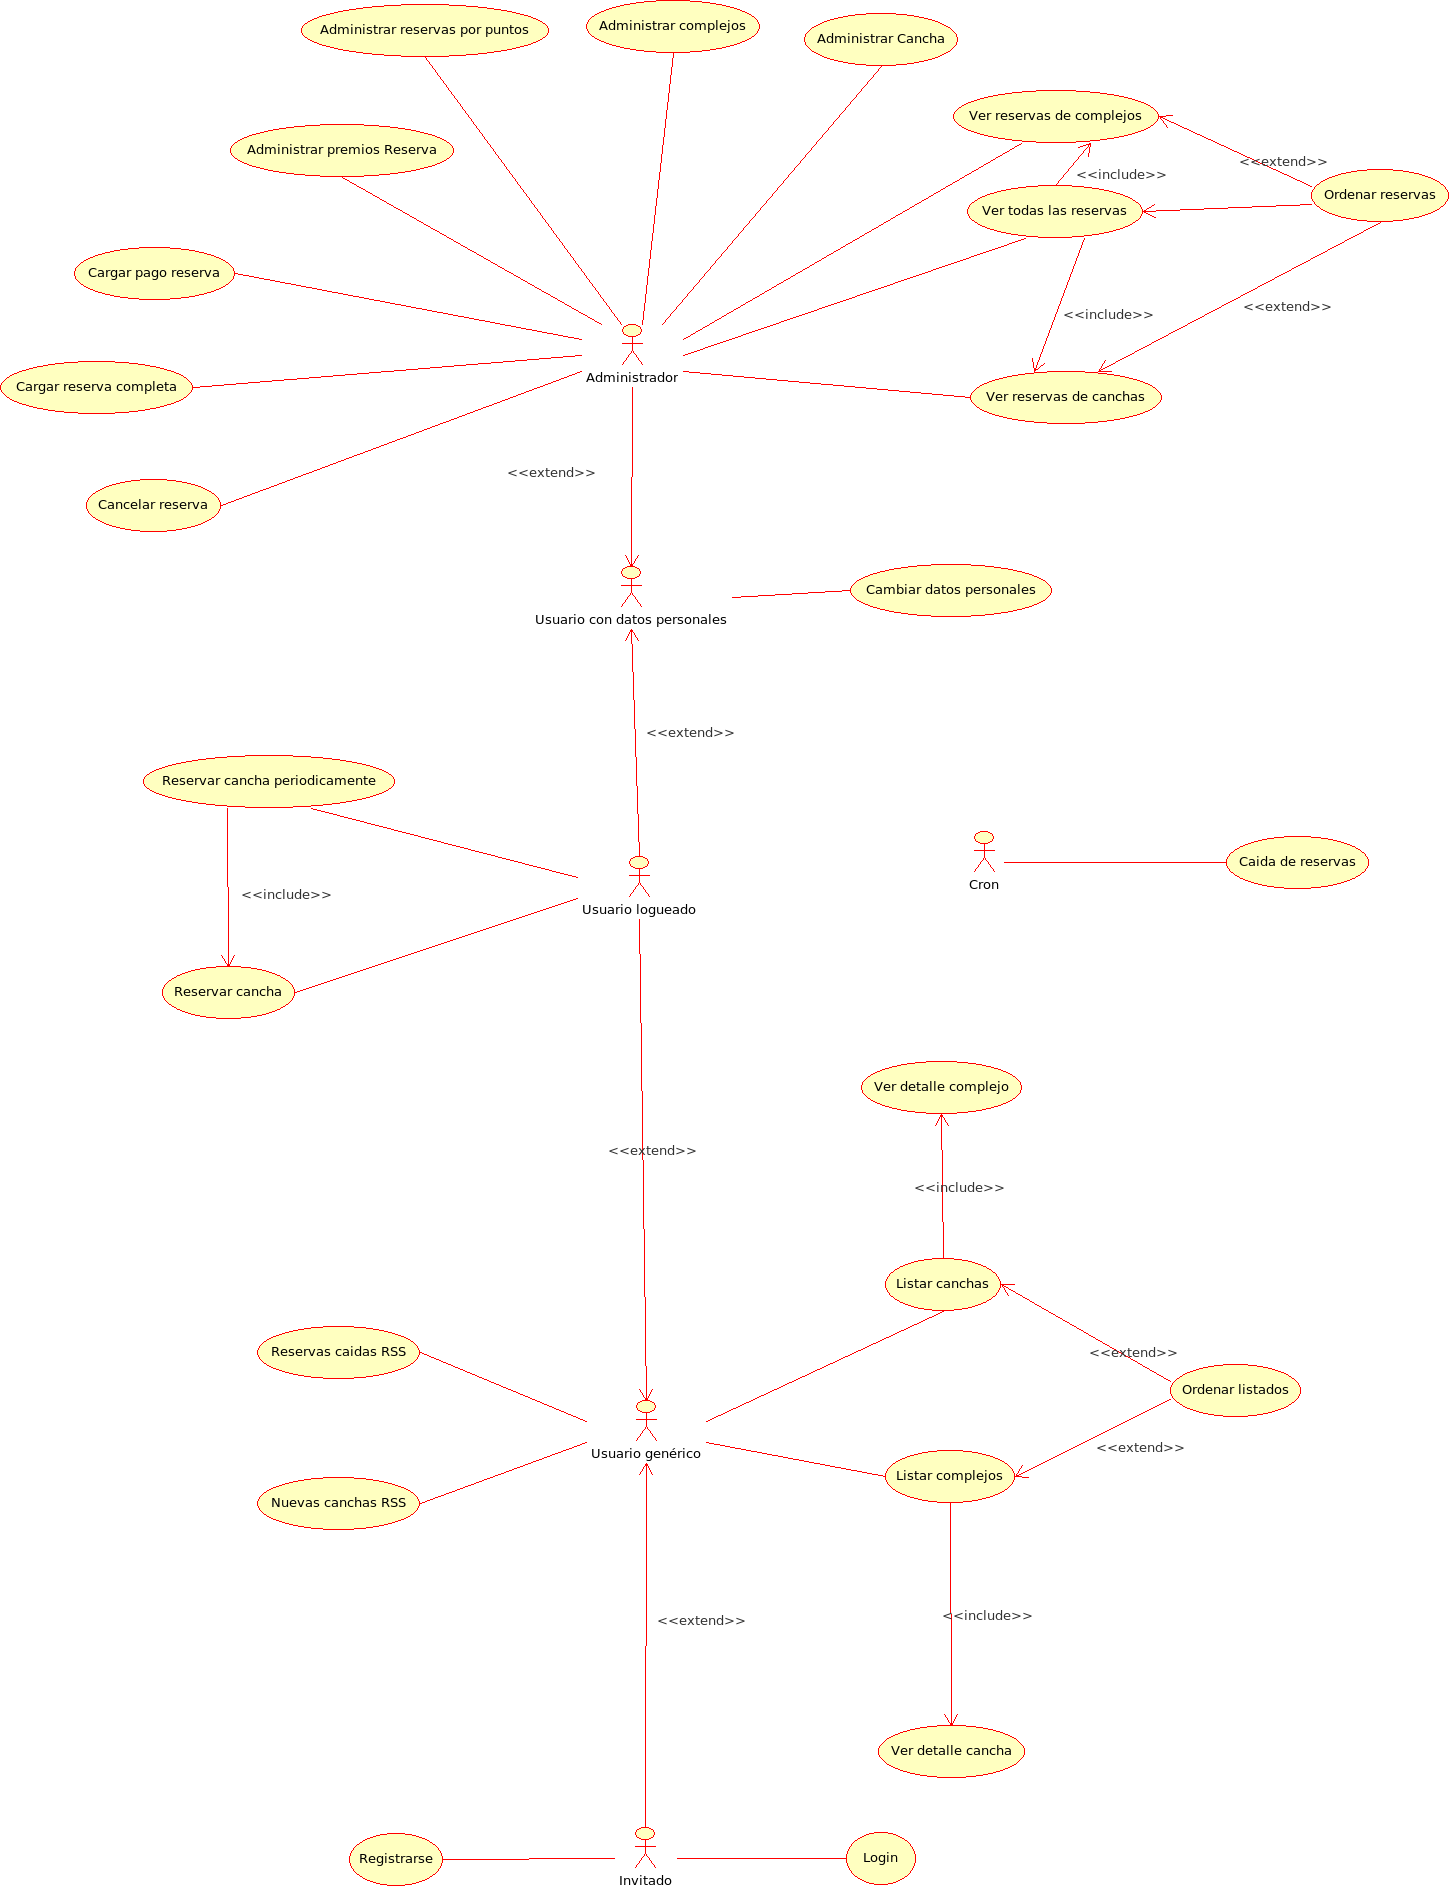
\includegraphics[width=1.00\textwidth]{use_cases.png}
 % use_cases.png: 1449x1890 pixel, 72dpi, 51.12x66.68 cm, bb=0 0 1449 1890
\end{center}

\pagebreak

\section{Casos de Uso}

% CAMBIAR DATOS PERSONALES
\subsection{Cambiar datos personales}
\begin{enumerate}

    \item
    \begin{enumerate}
    \item Descripción breve: \\
        Modificación de datos personales de un usuario genérico del sistema.
    \item Actores \\
        Usuario genérico.
    \item Disparadores: \\
        El usuario hace click en \emph{Perfil}
    \end{enumerate}

    \item Flujo de Eventos:
    \begin{enumerate}

        \item Flujo básico:
            \begin{enumerate}
                \item El usuario hace click en \emph{Perfil}.
                \item Cambia su direccion de mail o cantidad de dias de anticipacion con los que desea recibir un mail del sistema.
                \item Una vez realizados los cambios hace click en \emph{Confirmar}.
            \end{enumerate}
        \item Flujo alternativo:
            \begin{enumerate}
                \item Una vez realizados los cambios el usuario hace click en \emph{Cancelar}.
            \end{enumerate}
    \end{enumerate}

    \item Precondiciones: \\
        Usuario hizo \underline{Login} como usuario genérico.

    \item Post condiciones \\
        Datos personales del usuario guardados.

\end{enumerate}

% CAIDA DE RESERVAS
\subsection{Caida de reservas de canchas}
\begin{enumerate}

        \item
	\begin{enumerate}
            \item Descripción breve: \\
                Actualización de las reservas automáticamente cuando alguna reserva
                se da de baja por que se cumplió el tiempo de pago.
            \item Actores \\
                Cron.
            \item Disparadores: \\
                Dada una hora determina se ejecuta automáticamente.
        \end{enumerate}

        \item Flujo de Eventos: 

        \begin{enumerate}
            \item Flujo básico:
                Si existe alguna reserva cuyo tiempo de seña o pago expiró se da de baja.
        \end{enumerate}

        \item Precondiciones: \\
            Reserva existente.

        \item Post condiciones \\
            Reserva dada de baja.

\end{enumerate}

% RESERVAR CANCHA
\subsection{Reservar cancha}
\begin{enumerate}

    \item
    \begin{enumerate}
    \item Descripción breve: \\
        Este caso de uso describe la reserva de una cancha determinada.
    \item Actores \\
        Usuario genérico.
    \item Disparadores: \\
        El usuario hace click en \emph{Reservar} en el listado de canchas.
    \end{enumerate}

    \item Flujo de Eventos: 

    \begin{enumerate}

        \item Flujo básico:
		\begin{enumerate}
		\item	El usuario hace click en \emph{Reservar}.
		\item	El usuario hace click en el campo fecha.
		\item	Selecciona una fecha del calendario.
		\item	Selecciona un horario de la lista de horarios.		
		\item	El usuario hace click en \emph{Agregar}.
    		\end{enumerate}
    \end{enumerate}

    \item Precondiciones: \\
        Usuario hizo \underline{Login} como usuario genérico.
        La cancha está registrada en el sistema.
	La cancha tiene horarios disponibles.

    \item Post condiciones \\
        Cancha reservada para el usuario genérico.

\end{enumerate}

% RESERVAS CANCHA PERIODICAMENTE
\subsection{Reservar cancha periódicamente}
\begin{enumerate}

    \item
    \begin{enumerate}
    \item Descripción breve: \\
        Este caso de uso describe la reserva periódica de una cancha determinada.
    \item Actores \\
        Usuario genérico.
    \item Disparadores: \\
        El usuario hace click en \emph{Reservar} en el listado de canchas.
    \end{enumerate}

    \item Flujo de Eventos:

    \begin{enumerate}

        \item Flujo básico:
		\begin{enumerate}
		\item	El usuario hace click en \underline{Reservar} en el listado de canchas.
		\item	Hace click en \emph{Aqui} en el mensaje de informacion.
		\item	El usuario hace click en el campo fecha \emph{Desde}.
		\item	Selecciona una fecha del calendario.
		\item	El usuario hace click en el campo fecha \emph{Hasta}.
		\item	Selecciona una fecha del calendario.
		\item	Selecciona un horario de la lista de horarios.		
		\item	El usuario hace click en \emph{Agregar}.
		\end{enumerate}
	\end{enumerate}

    \item Precondiciones: \\
        Usuario hizo \underline{Login} como usuario genérico.
        La cancha está registrada en el sistema.

    \item Post condiciones \\
        Cancha reservada periódicamente para el usuario genérico.
	La cancha se reservara solo para los dias disponibles.
\end{enumerate}

% LISTAR CANCHAS
\subsection{Listar Canchas}
\begin{enumerate}

    \item
    \begin{enumerate}
    \item Descripción breve: \\
        Se le presenta al usuario un listado de las canchas cargadas en el sistema.
    \item Actores \\
        Usuario genérico.
    \item Disparadores: \\
        El usuario hace click en \emph{Canchas}.
    \end{enumerate}

    \item Flujo de Eventos:

    \begin{enumerate}

        \item Flujo básico:
        \begin{enumerate}
            \item El usuario hace click en \emph{Canchas}
            \item El sistema presenta al usuario un listado de las canchas.
        \end{enumerate}
    \end{enumerate}

    \item Precondiciones: \\
        No aplica.

    \item Post condiciones \\
        Listado de canchas presentado al usuario.

\end{enumerate}

% LISTAR COMLEJOS
\subsection{Listar Complejos}
\begin{enumerate}

    \begin{enumerate}
    \item Descripción breve: \\
        Se le presenta al usuario un listado de las complejos deportivos cargados en el sistema.
    \item Actores \\
        Usuario genérico.
    \item Disparadores: \\
        El usuario hace click en \emph{Complejos}.
    \end{enumerate}

    \item Flujo de Eventos: 

    \begin{enumerate}
        \item Flujo básico:
        \begin{enumerate}
            \item El usuario hace click en \emph{Complejos}
            \item El sistema presenta al usuario un listado de los complejos.
        \end{enumerate}
    \end{enumerate}

    \item Precondiciones: \\
        No aplica.

    \item Post condiciones \\
        Listado de complejos presentado al usuario.

\end{enumerate}

% ORDENAR LISTADO
\subsection{Ordenar Listado Cancha}
\begin{enumerate}

    \item
    \begin{enumerate}
    \item Descripción breve: \\
        Se le permite al usuario ordenar el listado de cancha segun diversos criterios.
    \item Actores \\
        Usuario genérico.
    \item Disparadores: \\
        El usuario realiza \underline{Listar Canchas}.
    \end{enumerate}

    \item Flujo de Eventos: 

    \begin{enumerate}

        \item Flujo básico:
        \begin{enumerate}
                    \item El usuario hace click en la columna \emph{Nombre}
			\begin{itemize}
			 \item Nombre
			 \item Complejo
			 \item Descripcion
			 \item Cantidad de Jugadores
			 \item Techada
			 \item Tipo de Piso
			 \item En Mantenimiento
			\end{itemize}
        \end{enumerate}
    \end{enumerate}

    \item Precondiciones: \\
        Listado cargado previamente.

    \item Post condiciones \\
        Listado ordenado segun criterio seleccionado.

\end{enumerate}

% VER DETALLE CANCHA
\subsection{Ver detalle cancha}
\begin{enumerate}

    \item
    \begin{enumerate}
    \item Descripción breve: \\
        Se muestra en detalle las características de una cancha.
    \item Actores \\
        Usuario generico.
    \item Disparadores: \\
        Click en el botón \emph{Ver detalles} dentro de \underline{Listar Canchas} o en \underline{Ver detalles complejo}
    \end{enumerate}

    \item Flujo de Eventos: 
    \begin{enumerate}
        \item Flujo básico:
        \begin{enumerate}
            \item El usuario selecciona \underline{Listar Canchas}
                o \underline{Ver detalles complejo} en el listado de complejos.
            \item El usuario hace click en \emph{Ver detalles}
            \item Se le presenta al usuario informacion detallada sobre la cancha seleccionada.
        \end{enumerate}
    \end{enumerate}

    \item Precondiciones: \\
        Usuario logueado como usuario común.
    \item Post condiciones \\
        Detalles de la cancha presentados al usuario.

\end{enumerate}

% ADMINISTRAR COMPLEJOS
\subsection{Administrar complejos}
\begin{enumerate}

    \item
    \begin{enumerate}
    \item Descripción breve: \\
        Este caso de uso describe las operaciones de creación, borrado y
        modificación de complejos.
    \item Actores \\
        Administrador.
    \item Disparadores: \\
        El administrador selecciona las operaciones explícitamente de su panel
        de administración.
    \end{enumerate}

    \item Flujo de Eventos: 

    \begin{enumerate}

        \item Flujo básico:
            El usuario selecciona \underline{Listar complejos}.
        \item Flujos alternativos:\\
            \begin{enumerate}
                \item \underline{Crear complejo} \\
                \begin{enumerate}
                    \item El usuario hace click en \textit{Crear nuevo complejo}
                    en el panel de administración.
                    \item El usuario completa los datos solicitados: País, 
                    provincia, localidad y barrio; teléfono, dirección, horario 
                    general de atención.
                    Se pueden indicar en forma opcional los rangos de puntos con
                    el vencimiento de los distintos estados de las canchas, el 
                    precio de las canchas y el porcentaje que corresponde a la
                    reserva.
                    \item El usuario da por finalizada la creación haciendo click
                    en \textit{Guardar complejo}.
                \end{enumerate}
                \item \underline{Modificar complejo} \\
                \begin{enumerate}
                    \item El usuario hace click en \textit{Modificar complejo} 
                    dentro de la entrada del listado que corresponde al complejo 
                    que desea modificar.
                    \item El usuario modifica los datos deseados.
                    \item El usuario da por finalizada la modificación haciendo 
                    click en \textit{Guardar complejo}.
                \end{enumerate}
                \item \underline{Borrar complejo}
                \begin{enumerate}
                    \item El usuario hace click en \textit{Borrar complejo}
                    dentro de la entrada del listado que corresponde al complejo
                     que desea eliminar.
                    \item El usuario confirma que desea eliminar el elemento
                    seleccionado.
                \end{enumerate}
            \end{enumerate}
    \end{enumerate}

    \item Precondiciones: \\
        Usuario hizo \underline{Login} como administrador.

    \item Post condiciones \\
        No aplica.

\end{enumerate}

% ADMINISTRAR CANCHAS
\subsection{Administrar canchas}
\begin{enumerate}

    \item
    \begin{enumerate}
    \item Descripción breve: \\
        Este caso de uso describe las operaciones de creación, borrado y
        modificación de canchas.
    \item Actores \\
        Administrador.
    \item Disparadores: \\
        El administrador selecciona las operaciones explícitamente de la página
        de administración de un complejo existente.
    \end{enumerate}

    \item Flujo de Eventos: 

    \begin{enumerate}

        \item Flujo básico:
            El usuario selecciona un complejo a través de 
            \underline{Listar complejos} y luego hace click en 
            \underline{Listar canchas}.
        \item Flujos alternativos:\\
            \begin{enumerate}
                \item \underline{Crear cancha} \\
                \begin{enumerate}
                    \item El usuario hace click en \textit{Crear nueva cancha}
                    en el listado de canchas del complejo elegido.
                    \item El usuario indica la cantidad de jugadores, el tipo de
                    piso y si la cancha es o no techada.
                    \item El usuario da por finalizada la creación haciendo click
                    en \textit{Guardar cancha}.
                \end{enumerate}
                \item \underline{Modificar cancha} \\
                \begin{enumerate}
                    \item El usuario hace click en \textit{Modificar cancha} 
                    dentro de la entrada del listado que corresponde a la cancha 
                    que desea modificar.
                    \item El usuario modifica los datos deseados.
                    \item El usuario da por finalizada la modificación haciendo 
                    click en \textit{Guardar cancha}.
                \end{enumerate}
                \item \underline{Borrar cancha}
                \begin{enumerate}
                    \item El usuario hace click en \textit{Borrar cancha}
                    dentro de la entrada del listado que corresponde a la cancha
                     que desea eliminar.
                    \item El usuario confirma que desea eliminar el elemento
                    seleccionado.
                \end{enumerate}
            \end{enumerate}
    \end{enumerate}

    \item Precondiciones: \\
        Usuario hizo \underline{Login} como administrador.

    \item Post condiciones \\
        No aplica.

\end{enumerate}

% ADMINISTRAR PREMIOS POR RESERVAS
\subsection{Administrar premios por reservas}
\begin{enumerate}

    \item
    \begin{enumerate}
    \item Descripción breve: \\
        Este caso de uso describe como se define la cantidad de puntos que gana
        un usuario al pasar por los distintos estados de una reserva, de acuerdo
        al sistema de puntos.
    \item Actores \\
        Administrador.
    \item Disparadores: \\
        El administrador hace click en \underline{Administrar premios por reserva}
        dentro de su panel de administración.
    \end{enumerate}

    \item Flujo de Eventos: 

    \begin{enumerate}

        \item Flujo básico:
            El usuario hace click en \underline{Administrar premios por reserva}.
            Luego determina cuantos puntos se otorgarán para las acciones de
            \textit{Reservar}, \textit{Señar} y \textit{Pagar}.
            También debe indicar cuántos puntos pierde el usuario si se cae
            su reserva, según ya estuviese reservada o señada.
    \end{enumerate}

    \item Precondiciones: \\
        Usuario hizo \underline{Login} como administrador.

    \item Post condiciones \\
        Todas las acciones tienen un puntaje asociado. Sistema de puntos
        actualizado.

\end{enumerate}

% ADMINISTRAR LIMITES DE RESERVAS POR PUNTOS
\subsection{Administrar límites de reservas por puntos}
\begin{enumerate}

    \item
    \begin{enumerate}
    \item Descripción breve: \\
        Este caso de uso describe como se definen los plazos de vencimiento de
        las reservas según el puntaje del usuario que haya realizado la reserva.
    \item Actores \\
        Administrador.
    \item Disparadores: \\
        El administrador hace click en 
        \underline{Administrar límites de reserva por puntos}
        dentro de su panel de administración.
    \end{enumerate}

    \item Flujo de Eventos: 

    \begin{enumerate}

        \item Flujo básico:
            El usuario hace click en \underline{Administrar límites de reserva
            por puntos}.
            Luego se determina cuales serán los plazos máximos de tiempo para la
            caducidad de cada complejo y cada cancha, teniendo en cuenta el rango
            de puntos que tenga el usuario.
    \end{enumerate}

    \item Precondiciones: \\
        Usuario hizo \underline{Login} como administrador.

    \item Post condiciones \\
        No aplica.

\end{enumerate}

% RESERVAR CAIDAS RSS
\subsection{RSS: Ver reservas caidas}
\begin{enumerate}
    \item
        \begin{enumerate}
            \item Descripción breve: \\
                Se listan los complejos con las últimas reservas caidas.
            \item Actores \\
                Usuario genérico, invitado.
            \item Disparadores: \\
                Acceso a la url del \emph{RSS} de reservas caidas.
        \end{enumerate}
    \item Flujo de Eventos:
        \begin{enumerate}
            \item Flujo básico:
		\begin{enumerate}                
		\item Usuario accede a la url del \emph{RSS} de reservas caidas.
        	\end{enumerate}
	\end{enumerate}
    \item Precondiciones: \\
        No aplica.
    \item Post condiciones \\
        Listado de reservas caidas con formato para ser leido por un lecto RSS.
\end{enumerate}

% NUEVAS CANCHAS RSS
\subsection{RSS: Ver nuevas canchas}
\begin{enumerate}

    \item
    \begin{enumerate}
        \item Descripción breve: \\
            Se listan las últimas canchas agregadas al sistema.
        \item Actores \\
            Usuario genérico, invitado.
        \item Disparadores: \\
            Acceso a la url del \emph{RSS} de canchas nuevas.
    \end{enumerate}

    \item Flujo de Eventos: 

        \begin{enumerate}
            \item Flujo básico:
        	\begin{enumerate}        
		\item 	Usuario genérico accede a la url del \emph{RSS} de canchas nuevas
	        \end{enumerate}
	\end{enumerate}

    \item Precondiciones: \\
        El lector del \emph{RSS} no necesita estar logueado como usuario.
    \item Post condiciones \\
        Listado de nuevas canchas con formato para ser leido con un lector RSS.

\end{enumerate}

% INVITADO CONFIRMAR REGISTRACION
\subsection{Invitado confirmar registración}
\begin{enumerate}

    \item
        \begin{enumerate}
            \item Descripción breve: \\
                Confirmar la registración para obtener efectivamente una cuenta de usuario del sistema.
            \item Actores \\
                Invitado.
            \item Disparadores: \\
                Click en el link del correo electrónico que se le envía al invitado.

        \end{enumerate}

    \item Flujo de Eventos:

        \begin{enumerate}
            \item Flujo básico:
                Un usuario genérico accede hace click en el link del correo electrónico que le fue enviado.

            \item Flujo alternativo:\\
                Se muestra un cartel que informa que los datos ingresados son
                incorrectos, puede volver a intentarlo.

                \begin{enumerate}
                    \item Condición 1 \\
                            El hash proporcionado no existe en la base de datos.
                    \item Condición 2 \\
                            Faltan datos requeridos.
                \end{enumerate}
    \end{enumerate}

    \item Precondiciones: \\
        No debe estar registrado como usuario del sistema.

    \item Post condiciones \\
        El invitado obtiene una cuenta de usuario y queda logueado en el sistema.

\end{enumerate}

% INVITADO REGISTRARSE
\subsection{Invitado registrarse}
\begin{enumerate}

    \item
        \begin{enumerate}
            \item Descripción breve: \\
                Obtener una cuenta de usuario del sistema.
            \item Actores \\
                Invitado.
            \item Disparadores: \\
                Click en \underline{registrarse} en la pantalla principal del sistema.

        \end{enumerate}

    \item Flujo de Eventos:

        \begin{enumerate}
            \item Flujo básico:
                Un usuario genérico accede a la pantalla principal del sistema y
                hace click en \underline{registrarse}. Ingresa los datos necesarios
                para registrarse como usuario del sistema.

            \item Flujo alternativo:\\
                Se muestra un cartel que informa que los datos ingresados son
                incorrectos, puede volver a intentarlo.

                \begin{enumerate}
                    \item Condición 1 \\
                            El usuario ingresado ya existe dentro del sistema.
                    \item Condición 2 \\
                            Faltan datos requeridos.
                    \item Condición 3 \\
                            Las contrase\~nas ingresadas no son iguales.
                    \item Condición 4 \\
                            Alguna combinación de las anteriores.
                \end{enumerate}
	\end{enumerate}

    \item Precondiciones: \\
        No debe estar registrado como usuario del sistema.

    \item Post condiciones \\
        Se envía un correo elecrtónico al usuario para confirmar su casilla.


\end{enumerate}

% INVITADO LOGIN
\subsection{Invitado login}
\begin{enumerate}

    \item
        \begin{enumerate}
            \item Descripción breve: \\
                Acceso al sistema como usuario.
            \item Actores \\
                Invitado.
            \item Disparadores: \\
                El invitado hace click en \emph{Ingresar}
        \end{enumerate}

    \item Flujo de Eventos:
        \begin{enumerate}
            \item Flujo básico:
        	\begin{enumerate}
		\item	El invitado accede al sitio.
                \item 	El invitado ingresa nombre de usuario, contraseña. 
		\end{enumerate}
            \item Flujo alternativo:\\
		\begin{enumerate}
		\item	El usuario inserta datos invalidos.
		\item 	El sistema prohibe la entrada al sitio e informa al usuario del hecho.
		\end{enumerate}
        \end{enumerate}
        \item Precondiciones: \\
            Debe estar registrado como usuario del sistema.
        \item Post condiciones \\
            El usuario tiene acceso al sistema.
\end{enumerate}

% CARGAR PAGO POR RESERVAS
\subsection{Cargar pago reservas}
\begin{enumerate}
    \item
    \begin{enumerate}
    \item Descripción breve: \\
        Se carga un pago para una determinada reserva.
    \item Actores \\
        Administrador.
    \item Disparadores: \\
        Click en el botón \emph{Cargar Pago} dentro de la
        página que muestra las reservas.
    \end{enumerate}

    \item Flujo de Eventos: 

    \begin{enumerate}

        \item Flujo básico:
	\begin{enumerate}
            \item Administrador hace click en \underline{Reservas}. 
	    \item El Administrador hace click en \emph{Cargar Pago}. 
	    \item Ingresa el monto que fue pagado de la reserva.
	\end{enumerate}

        \item Flujos alternativos:\\
            Se muestra un cartel que informa que la cantidad ingresada es
            incorrecta.
            \begin{enumerate}
                \item Condición 1 \\
                    La cantidad ingresada es incorrecta.
            \end{enumerate}

    \end{enumerate}

    \item Precondiciones: \\
        Ususario logueado como administrador.

    \item Post condiciones \\
        Pago de la reserva cargado y, si aplica, estado de la reserva y puntos
        del usuario que emitió la reserva actualizados.

\end{enumerate}

% CARGAR RESERVA COMPLETA
\subsection{Cargar reserva completa}
\begin{enumerate}

    \item
    \begin{enumerate}
    \item Descripción breve: \\
        Se carga un pago completo para una determinada reserva.
    \item Actores \\
        Administrador.
    \item Disparadores: \\
        Click en el botón \emph{Cargar Pago Completo} dentro de la página que muestra las reservas.
    \end{enumerate}

    \item Flujo de Eventos:

    \begin{enumerate}

        \item Flujo básico:
	\begin{enumerate}
            \item Administrador hace click en \underline{Reservas}. 
	    \item El Administrador hace click en \emph{Cargar pago completo de reserva}.
	\end{enumerate}
    \end{enumerate}

    \item Precondiciones: \\
        Ususario logueado como administrador.

    \item Post condiciones \\
        Pago de la reserva cargado y estado de la reserva actualizado a pagada.
        Puntos del usuario que emitió la reserva actualizados.

\end{enumerate}


% VER DETALLE COMPLEJO
\subsection{Ver detalle complejo}
\begin{enumerate}

    \item
    \begin{enumerate}
    \item Descripción breve: \\
        Se muestra en detalle las características de un complejo.
    \item Actores \\
        Usuario generico, Invitado, Administrador.
   \item Disparadores: \\
        Click en el botón \emph{Detalles} dentro de la
        página que lista los complejos del sistema.
    \end{enumerate}

    \item Flujo de Eventos:

    \begin{enumerate}

        \item Flujo básico:
	\begin{enumerate}
        	\item El actor hace click en \underline{Complejos}. 
		\item El actor hace click en \emph{Detalles}.
	\end{enumerate}

    \end{enumerate}

    \item Precondiciones: \\
        No aplica.

    \item Post condiciones \\
        Vista detallada de la informacion del complejo.

\end{enumerate}

% VER TODAS LAS RESERVAS
\subsection{Ver todas las reservas}
\begin{enumerate}

    \item
    \begin{enumerate}
    \item Descripción breve: \\
        Se listan todas las reservas existentes.
    \item Actores \\
        Administrador.
    \item Disparadores: \\
        Click en el botón \underline{Reservas}.
    \end{enumerate}

    \item Flujo de Eventos: 

    \begin{enumerate}

        \item Flujo básico:
    		\begin{enumerate}
            	\item Un Administrador hace click en \emph{Reservas}.
		\end{enumerate}
    \end{enumerate}

    \item Precondiciones: \\
        Usuario logueado como administrador.

    \item Post condiciones \\
        Listo de reservas presentado al actor.

\end{enumerate}

% VER RESERVAS DE CANCHA
\subsection{Ver reservas de canchas}
\begin{enumerate}

    \item
    \begin{enumerate}
    \item Descripción breve: \\
        Se listan las reservas de canchas.
    \item Actores \\
        Administrador.
    \item Disparadores: \\
        Click en el botón \underline{Canchas}.
    \end{enumerate}

    \item Flujo de Eventos:

    \begin{enumerate}

        \item Flujo básico:
		\begin{enumerate}
            	\item	Un Administrador hace click en \underline{Reservas}.
		\item	El Administrador hace click en \emph{Ver Reservas}.
		\end{enumerate}
    \end{enumerate}

    \item Precondiciones: \\
        Administrador logueado como administrador.

    \item Post condiciones \\
        Listado de reservas para la cancha seleccionada.

\end{enumerate}

% VER RESERVAS DE COMPLEJO
\subsection{Ver reservas de complejos}
\begin{enumerate}

    \item
    \begin{enumerate}
    \item Descripción breve: \\
        Se listan las reservas de un complejo.
    \item Actores \\
        Administrador.
    \item Disparadores: \\
        Click en el botón \emph{Ver reservas}
        en el listo de complejos.
    \end{enumerate}

    \item Flujo de Eventos:

    \begin{enumerate}

        \item Flujo básico:
	\begin{enumerate}
            \item Un Administrador hace click en \underline{Complejos}.
	    \item El Administrador hace click en \emph{Ver Reservas} para un determinado complejo.
        \end{enumerate}

    \end{enumerate}

    \item Precondiciones: \\
        Administrador logueado como administrador.

    \item Post condiciones \\
        Listado de las reservas para un determinado complejo.

\end{enumerate}

% ORDENAR RESERVAS
\subsection{Ordenar reservas}
\begin{enumerate}

    \item
    \begin{enumerate}
    \item Descripción breve: \\
        Se ordenan los listados de reservas.
    \item Actores \\
        Administrador.
    \item Disparadores: \\
        Click en el botón en el nombre de cualquier columna
        dentro de cualquier listado de reservas.
    \end{enumerate}

    \item Flujo de Eventos: 

    \begin{enumerate}

        \item Flujo básico:
	\begin{enumerate}
            \item Un Administrador hace click en \underline{Reservas}
	    \item El Administrador hace click en alguno de los nombres de las columnas, el cual sera el criterio de ordenacion.
Estos pueden ser:
	\begin{itemize}
	 \item Usuario
	\item Cancha
	\item Complejo
	\item Estado
	\item Costo
	\item Pagado
	\end{itemize}
	\end{enumerate}

    \item Precondiciones: \\
        \begin{enumerate}
            \item Administrador logueado como administrador.
        \end{enumerate}

    \item Post condiciones \\
        Listado ordenado segun columna seleccionada.

\end{enumerate}

\end{document}
